\section{Userverwaltung [L]}
\setauthor{Litzlbauer Lorenz}
Im Projekt wurde eine Userverwaltung eingebaut. Der*die User*in kann sich auf der Weboberfläche anmelden und registrieren. Je nach Registrierungsstatus (bestehende Anmeldung oder nicht) stehen mehr oder weniger Funktionalitäten zur Verfügung. Ein*e Besucher*in, die nicht angemeldet ist, kann alle Ausstellungen ansehen und auf der Suchunterseite nach Ausstellungen suchen. Ein*e registrierte*er User*in kann zusätzlich auch seine*ihre Profileseite sehen und Ausstellungen selbst erstellen und veröffentlichen. Die Navigationsleiste wurde so programmiert, dass sie dem*der User*in nur die Unterseiten zeigt, die diese durch ihrem Registrierungsstatus auch besuchen kann. 

Im folgendem Abschnitt 'Sign-, Log-In Funktionalitäten' wird die Implementation des Userverwaltung und die damit verbundenen Features erklärt. 

\subsection{Implementation im Frontend [L]}
\setauthor{Litzlbauer Lorenz}
Nachdem der Json-Web-Token im Backend implementiert wurde, galt es diesen auch auf dem Frontend einzubauen. Der Json-Web-Token dient zur Authentifizierung des*der User*in und zum rollenbasierenden Schutz der API. 

\subsubsection{Sign-In und Login}
Da der Json-Web-Token als Beweis dafür dient, dass der*die User*in authentifiziert ist, muss sich der*die Benutzer vor dem Erhalten des Token dafür erst auf der Weboberfläche registrieren oder anmelden. 

\begin{figure}
    \centering
    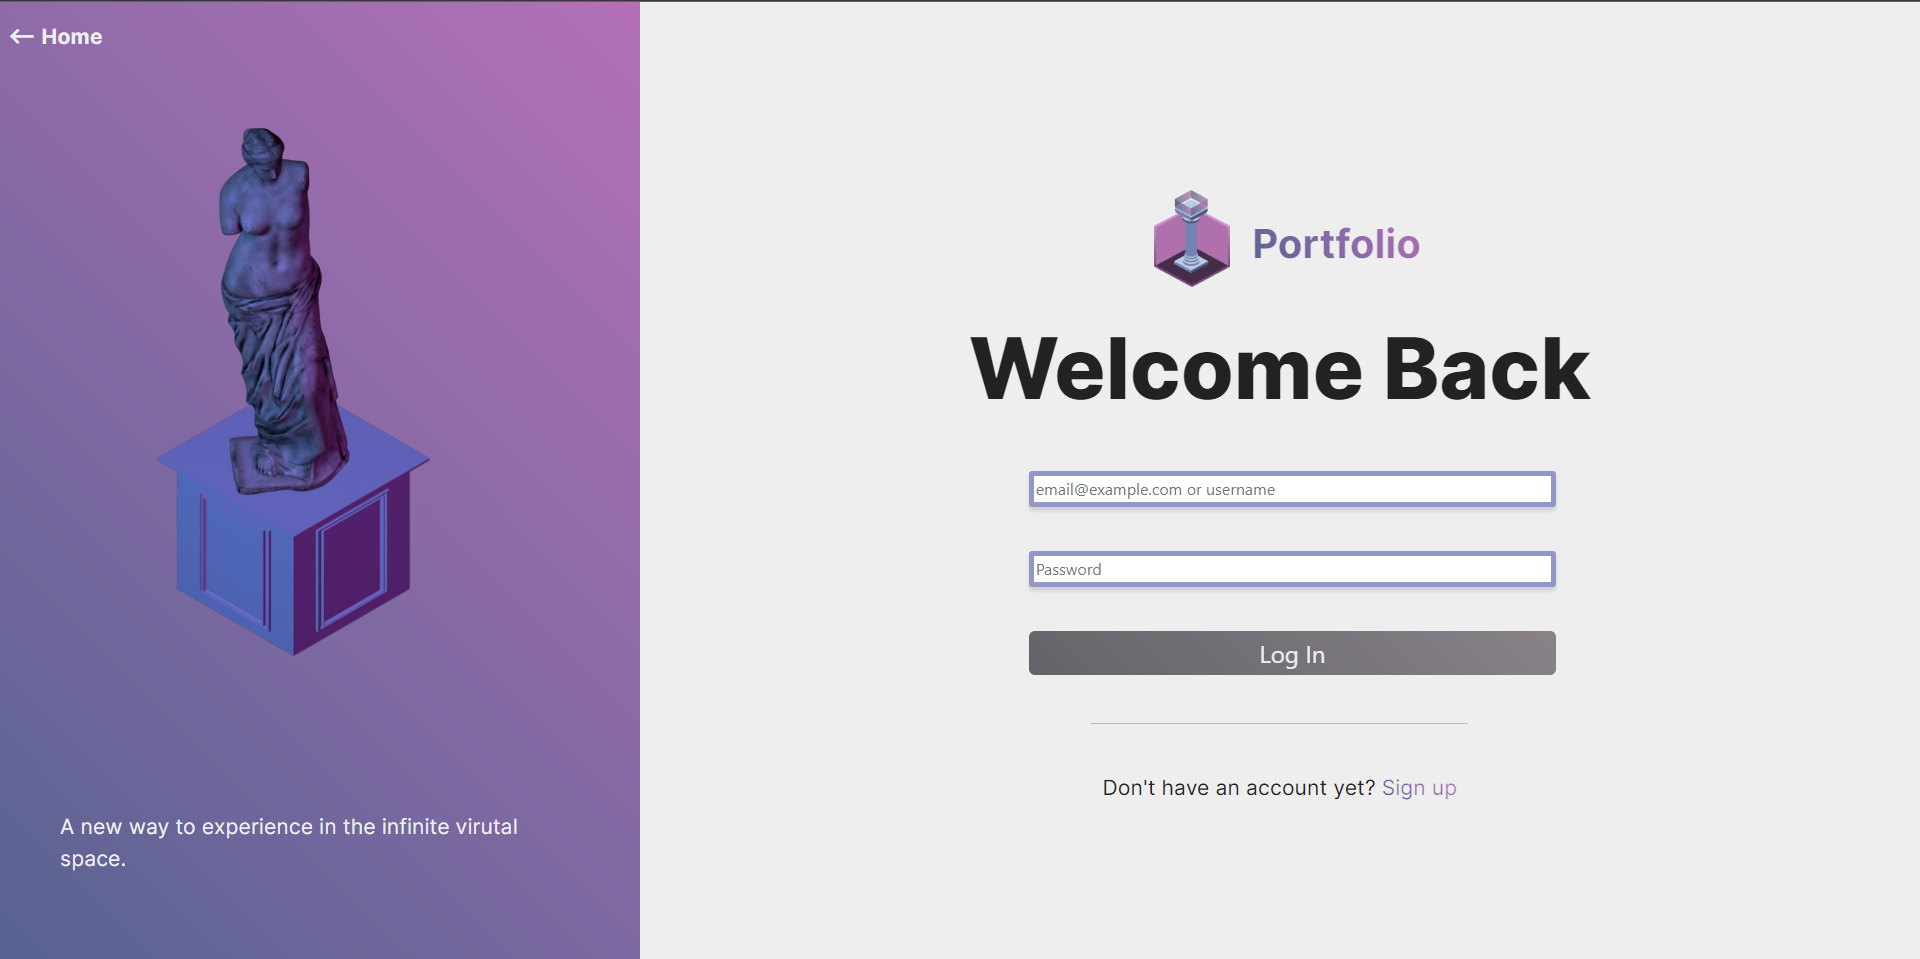
\includegraphics[scale=0.25]{pics/GalleryLogIn.png}
    \caption{Projekt: Login Page}
    \label{fig:impl:login}
\end{figure}

Für das User-Interface ist eine Anmelde- und Registrierungsfunktionalität implementiert worden (siehe Abbildung \ref{fig:impl:login}). Die Anmelde- und Registrierungsfelder wurden mithilfe von reaktiven Formularen und Validatoren (siehe \ref{par:impl:usermanagment:reactiveForms}) umgesetzt.
Die Validatoren bestimmen, dass ein Passwort mindestens 8 Zeichen besitzen muss, um akzeptiert zu werden.

Nachdem vom User eine valide Eingabe getätigt wurde, aktiviert sich der Anmelde- bzw. Registrierungsbutton und lässt sich betätigen.

Bei der Aktivierung ändert sich die Farbe des Buttons von Grau auf einen bunten blauen pinken Farbverlauf, um ein visuelles Feedback an den*die Benutzer*in zu senden. Nachdem der*die User*in die Eingabe bestätigt hat, indem sie*er die Schaltfläche drückt, werden die Anmeldedaten über das HTTPS-Protokoll mithilfe des HTTP-Moduls (siehe \ref{sec:HTTPModule}) an den Server gesendet. Nach einer erfolgreichen Anmeldung bzw. Registrierung wird an die Weboberfläche eine Antwort geschickt, in der der Json-Web-Token enthalten ist. Danach wird der*die User*in auf die Profilseite weitergeleitet. Bei einem gescheiterten Anmelde- bzw. Registrierungsversuch wird der*die User*in durch eine Fehlermeldung informiert.

Nach der erfolgreichen Anmeldung bzw. Registrierung wird vom Server ein Json-Web-Token ausgestellt. Bei einem HTTP-Request vom Client zum Server kann der Json-Web-Token im Header des Requests platziert werden. Der Server kann kann diesen auslesen und so feststellen, ob ein*e Benutzer*in auch wirklich authentifiziert ist.

Nun gibt es aber mehrere Nachteile, die aus diesem Prozess entstehen. Der*Die User*in muss bei jedem neuen Besuch der Seite sowie bei einem Reload neu anmelden. Im Code muss bei jedem HTTP-Request (also jeder Kommunikation mit dem Server) der Json-Web-Token manuell in dem Header platziert werden. Dadurch entsteht im Code eine hohe Redundanz. Im folgenden Kapitel "Token-Verwaltung" (siehe \ref{sec:tokenveraltung}) und "HTTP-Interceptoren" (siehe \ref{sec:httpinterceptor}) wird beschrieben, wie mit diesen Problemen umgegangen wurde.

\paragraph{Formulare und Validation}
\label{par:impl:usermanagment:reactiveForms}
In Webanwendungen gibt es zahlreiche Formulare, die als eine der primären Kommunikationsschnittstellen zum Besucher*in dienen. Es gibt dafür die nativen HTML-Inputelemente, aber zu einer guter User-Experience gehört auch ein visuelles Feedback für den*die Benutzer*in bei Bearbeitung eines Formulars. Der Entwicklungsaufwand wächst allerdings mit der Anzahl der im Formular eingefügten Features.

Angular bietet verschiedene Implementierungsarten, um die visuelle Komponenten umzusetzen und den Entwicklungsaufwand zu minimieren. Bei diesen Ansätzen können mehrere Eingabedaten zentral ausgewertet und weiterverarbeitet werden und der Status des Formulars bei Änderungen und Fehlern visuell dargestellt werden. \cite[Bookmonkey - 12 Formularverarbeitung und
Validierung: Iteration IV]{AngularBuch}

Bei den Ansätzen unterscheidet man zwischen den reactiven Forms und den Template-Driven-Forms.

\subsubsection{Token-Verwaltung}
\label{sec:tokenveraltung}
Um das Problem, dass beim neu Laden der Webseite der Anmeldestatus bzw. der Json-Web-Token verloren geht, zu lösen, wird der Json-Web-Token im Locale-Storage des Browsers gespeichert. 
Im Codeausschnitt (siehe \ref{lst:impl:sign:jwtLocalstorage}) ist ein Teil des Authentifizierungsdienstes des Projektes zu sehen. Mit der Funktion \emph{setSaveJWT} wird der ausgestellte Json-Web-Token ausgelesen und die darin enthaltenen Informationen, der Name und die Id des Benutzers, die Id des Tokens und das Ablaufdatum des Tokens im Locale-Storage (siehe im Absatz WebStorage API \ref{par:impl:usermanagment:WebStorage}) gespeichert, damit die Daten auch nach dem neu Laden der Webseite erhalten bleiben. Die Funktion \emph{isLoggedIn} gibt nach dem Aufruf den Status mit, ob eine Person angemeldet ist oder nicht. Dafür benutzt die Funktion das im Json-Web-Token enthaltene Ablaufdatum und vergleicht es mit dem aktuellen Datum. Zuletzt gibt es noch die \emph{logout} Funktion, diese löscht die im Locale-Storage enthaltenen Json-Web-Token-spezifischen Daten.

\begin{lstlisting}[caption=auth.service.ts - Json-Web-Token und Localstorage,label=lst:impl:sign:jwtLocalstorage,language=TypeScript ]
export class AuthService {
    ...
    setSaveJWT(value: any) {
        let decodedJWTPayload = JSON.parse(atob(value.split('.')[1]))
        localStorage.setItem("user", decodedJWTPayload.sub)
        localStorage.setItem('id_token', value)
        localStorage.setItem('expires_at', decodedJWTPayload.exp)
        localStorage.setItem('user_id', decodedJWTPayload.userid)
      }

    isLoggedIn(): boolean {
        if (localStorage.getItem('id_token') && localStorage.getItem('expires_at')) {
          let temp = new Date().getTime()
          const exp = Number(localStorage.getItem('expires_at'))
          return temp < exp
        } else {
          return false;
        }
      }

    logout() {
        localStorage.removeItem("user")
        localStorage.removeItem('id_token')
        localStorage.removeItem('expires_at')
        localStorage.removeItem('user_id')
      }
    ...
}        
\end{lstlisting}

\paragraph{WebStorage API}
\label{par:impl:usermanagment:WebStorage}
Das WebStorage API bietet verschiedene Möglichkeiten, Daten per Schlüssel-Werte-Paare im Web zu persistieren. Persistenz ist die Fähigkeit, Daten in einem nicht flüchtigen Speicher zu speichern, um so den Datenverlust beim Neustart des Systems zu verhindern. Das WebStorage API ist nicht Teil des DOM, sondern der globalen Web-Variable window. Die zwei Arten, Daten mittels der WebStorage API zu persistieren, sind der Locale-Storage und der Session-Storage.
\cite{WikiPersistenzDefinition} \cite{WebStorageAPI}


\subparagraph{Session-Storage}
Daten im Session-Storage werden je nach ihrem Ursprung getrennt aufbewahrt. Sie werden für die Zeit der Webseitensession gespeichert, wenn der Browser oder der Tab geschlossen wird, werden die Information gelöscht.
\cite{WebStorageAPI}

\subparagraph{Local-Storage}
Daten werden wie im Session-Storage persistiert, die Daten bleiben nach den Schließen des Browsers oder Tabs erhalten. Die Daten können nur durch JavaScript oder das Löschen des Webbrowser-Caches gelöscht werden.
\cite{WebStorageAPI}

\subparagraph{Allgemeine Informationen}
Beide Speichermethoden benutzen keine Server, um die Daten zu speichern, sondern den Cache des Webbrowsers. Das Speicherlimit hängt vom Webbrowser ab, doch beträgt es mndesten 5 MB und es können nur Zeichenketten gespeichert werden.
\cite{WebStorageAPI}

\subsubsection{HTTP-Interceptoren}
\label{sec:httpinterceptor}
HTTP-Interceptoren funktionieren in Angular als Zwischenschicht zwischen ausgehenden HTTP-Abfragen und eingehenden HTTP-Antworten und können diese manipulieren.
 HTTP-Interceptoren werden auf jeden Request angewendet. Es ist somit das perfekte Werkzeug, um in allen HTTP-Requests den JWT in den Header zu verpacken.
\cite[10.3 Interceptoren: HTTP-Requests abfangen und transformieren]{AngularBuch}

Wird ein Request an den Server gesendet, wird die Verarbeitung vom Interceptor unterbrochen. Es wird überprüft, ob der Json-Web-Token verfügbar ist. Wenn das zutrifft, wird der ursprüngliche Request geklont und in der Authentifizierungsspalte des Headers wird die Json-Web-Token-Id hinzugefügt. Danach wird der Request wieder zum Server weitergeleitet (siehe Code \ref{lst:impl:sign:JWTInterceptor}). 

\begin{lstlisting}[caption=auth.interceptor.ts - add JWT to Request Header,label=lst:impl:sign:JWTInterceptor,language=TypeScript]
import { Injectable } from '@angular/core';
import {
  HttpRequest,
  HttpHandler,
  HttpEvent,
  HttpInterceptor
} from '@angular/common/http';
import { Observable } from 'rxjs';

@Injectable()
export class AuthInterceptor implements HttpInterceptor {

  constructor() {}

  intercept(request: HttpRequest<unknown>, next: HttpHandler): Observable<HttpEvent<unknown>> {

    const idToken = localStorage.getItem('id_token')
    if (idToken) {
      const cloned = request.clone(
        {
          headers: request.headers.set('Authorization', 'Bearer '.concat(idToken))
        }
      )

      return next.handle(cloned)
    }

    return next.handle(request);
  }
}
\end{lstlisting}

\subsubsection{Routing- und Navigations-Einschränkung}
Zum Start dieses Entwicklungsschrittes war der Interceptor und die JWT Verwaltung fertig. Doch das Projekt brauchte eine besseres visuelles Feedback System um dem*der Kunden*in den Anmeldestatus zu zeigen.

Deswegen und um zu verhindern das Benutzer*in auf Unterseiten sind auf denen sie wegen ihres Registrationsstatus (noch nicht authentifiziert) noch nichts machen können, wurde je nach Anmeldestatus andere Routen und Informationen auf der Navigationsbar gezeigt (siehe Abbildung \ref{fig:impl:navbarvergleich}). Dafür wurde die Navigationsleistenlogik und die Navigationsleistenservice angepasst. Zusätzlich wurde AuthGuard verwendet um Routen zu sperren auf, die der*die Benutzer*in wegen dem Registrationsstatus noch keinen Zugriff hat. 

\begin{figure}
  \centering
  \includegraphics[scale=0.5]{pics/navbarRequistrationsstatusGegenüberstellung.png}
  \caption{Navbar: authentifiziert vs noch nicht authentifiziert}
  \label{fig:impl:navbarvergleich}
\end{figure}


\subsection{Erledigte User-Stories [L]}
Im Entwicklungsprozess des Usermanagment-System wurden folgende User-Stories vollendet: 
\begin{compactenum}
  \item Als Designer möchte ich einen Login, um meine Ausstellungen speichern und im Nachhinein immer öffnen zu können.
  Akzeptanzkriterien:
  \begin{compactitem}
      \item Man kann sich neu registrieren
      \item Registrierung mittels Username und Passwort
      \item Das Passwort muss überprüft werden beim Erstellen und mind. 8 Zeichen enthalten
  \end{compactitem}
  \item Als User*in will ich andere Rechte haben, je nachdem ob ich angemeldet bin oder nicht. Akzeptanzkriterien:
  Wenn ein*e User*in angemeldet ist, kann er*sie:
      \begin{compactitem}
          \item Ausstellungen ansehen
          \item Ausstellungen erstellen/löschen
      \end{compactitem}  
  Wenn ein ein*e User*in nicht angemeldet ist, kann er*sie:
      \begin{compactitem}
          \item Ausstellungen ansehen
          \item keine Ausstellungen erstellen
          \item keine Ausstellungen favorisieren
      \end{compactitem} 
\end{compactenum}